\documentclass[11pt]{article}
\usepackage{tikz}
\usepackage{amssymb}
\usepackage{geometry}
\geometry{letterpaper, landscape, margin=0.4in}
\usetikzlibrary{positioning, calc}

% Door macros
\newcommand{\hdoor}[2]{%
  \fill[white,draw=black,thick] ({#1-0.1},{#2-0.12}) rectangle ({#1+0.1},{#2+0.12});%
}
\newcommand{\vdoor}[2]{%
  \fill[white,draw=black,thick] ({#1-0.12},{#2-0.1}) rectangle ({#1+0.12},{#2+0.1});%
}

\begin{document}

\begin{center}
{\Huge \textbf{The Grain Mother's Ruin}}\\[0.3em]
{\Large Level 5 --- The Inner Sanctum | 5 Keyed Areas}
\end{center}

\vspace{0.3em}

\begin{center}
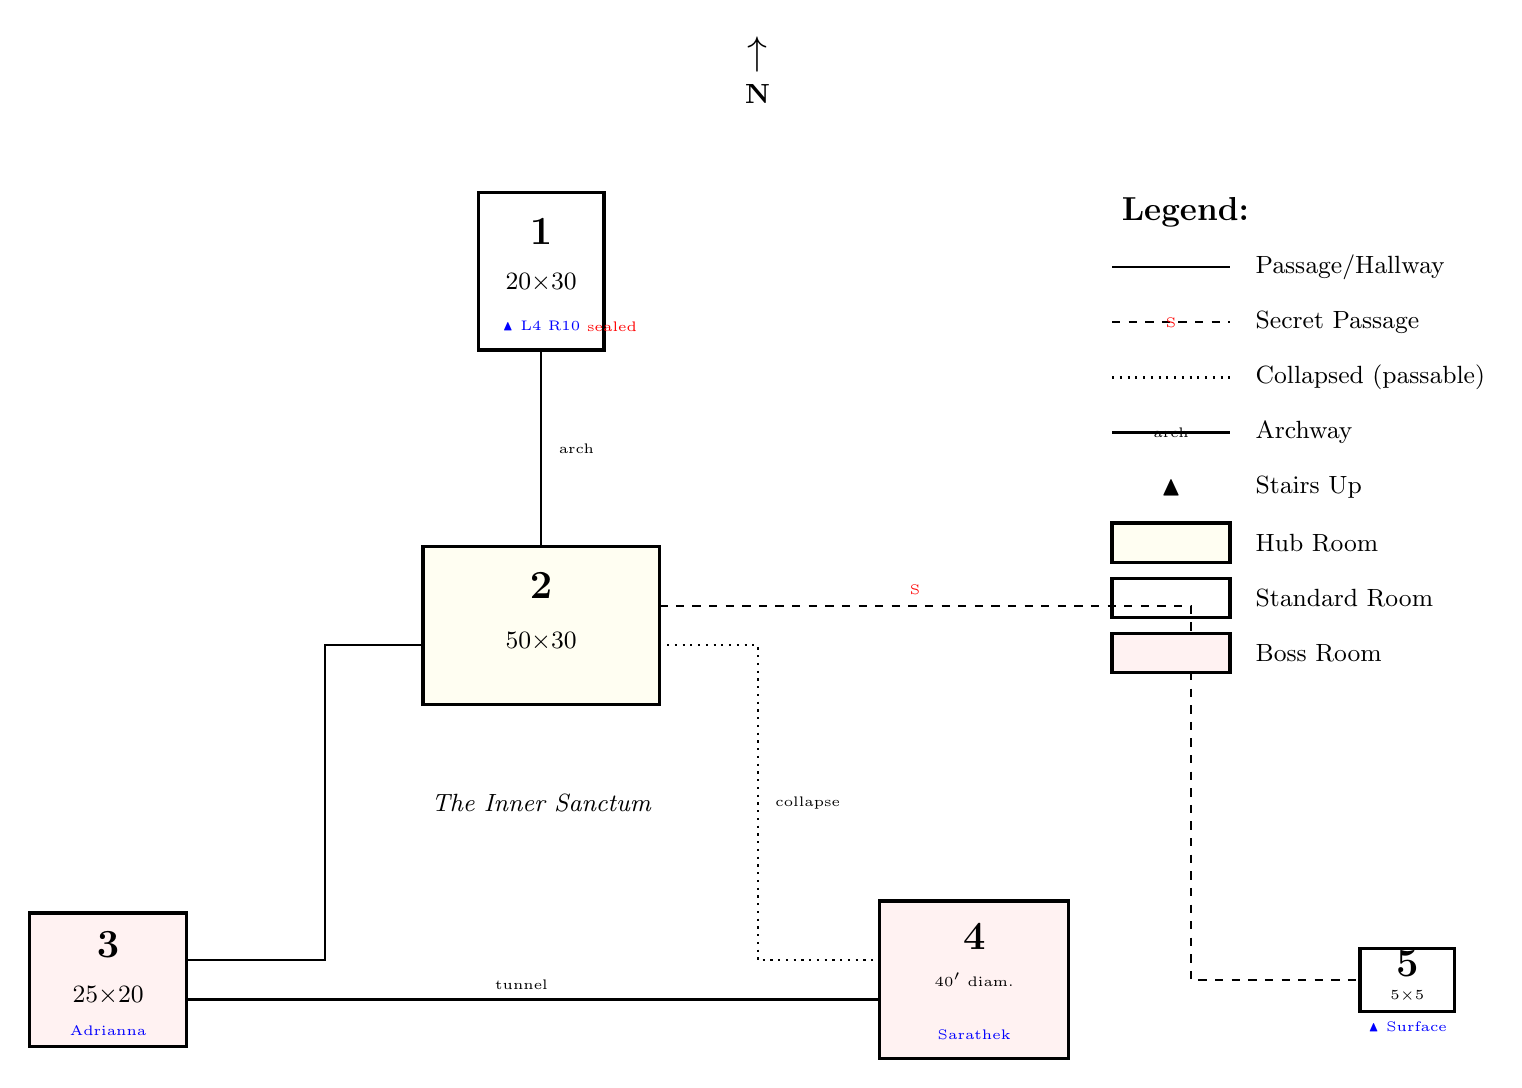
\begin{tikzpicture}[
    room/.style={draw, very thick, rectangle},
    hub/.style={draw, very thick, rectangle, fill=yellow!5},
    boss/.style={draw, very thick, rectangle, fill=red!5},
    connection/.style={draw, thick},
    secret/.style={dashed, thick},
    trap/.style={red},
    scale=1.0
]

% ============================================================
% GRID PARAMETERS
% CellW=3.5, CellH=2.5, Gutter=2.0
% Cols: c0(x=1.75) c1(x=7.25) c2(x=12.75) c3(x=18.25)
% Rows: r0(y=1.25) r1(y=5.75) r2(y=10.25)
% Vertical gutters: c0-c1(x=4.5) c1-c2(x=10.0) c2-c3(x=15.5)
% Horizontal gutters: r0-r1(y=3.5) r1-r2(y=8.0)
% ============================================================

% ============================================================
% NORTH ARROW
% ============================================================
\node at (10.0, 13.0) {\Large $\uparrow$};
\node at (10.0, 12.5) {\textbf{N}};

% ============================================================
% Room 1: The Threshold (20x30 ft)
% Cell: (c1, r2) -> center (7.25, 10.25)
% Rect: (6.45, 9.25) to (8.05, 11.25)
% ============================================================
\draw[room] (6.45,9.25) rectangle (8.05,11.25);
\node at (7.25,10.75) {\Large \textbf{1}};
\node[font=\small] at (7.25,10.1) {20$\times$30};
\node[blue,font=\tiny] at (7.25,9.55) {$\blacktriangle$ L4 R10};
\node[red,font=\tiny] at (8.15,9.55) {sealed};

% ============================================================
% Room 2: The Desecrated Gallery (50x30 ft) -- HUB: 4 connections
% Cell: (c1, r1) -> center (7.25, 5.75)
% Rect: (5.75, 4.75) to (8.75, 6.75)
% ============================================================
\draw[hub] (5.75,4.75) rectangle (8.75,6.75);
\node at (7.25,6.25) {\Large \textbf{2}};
\node[font=\small] at (7.25,5.55) {50$\times$30};

% ============================================================
% Room 3: Adrianna's Sanctum (25x20 ft) -- BOSS: Adrianna
% Cell: (c0, r0) -> center (1.75, 1.25)
% Rect: (0.75, 0.4) to (2.75, 2.1)
% ============================================================
\draw[boss] (0.75,0.4) rectangle (2.75,2.1);
\node at (1.75,1.7) {\Large \textbf{3}};
\node[font=\small] at (1.75,1.05) {25$\times$20};
\node[blue,font=\tiny] at (1.75,0.6) {Adrianna};

% ============================================================
% Room 4: The Fountain of Demeter (40' diameter, circular) -- BOSS: Sarathek
% Cell: (c2, r0) -> center (12.75, 1.25)
% Rect: (11.55, 0.25) to (13.95, 2.25)
% ============================================================
\draw[boss] (11.55,0.25) rectangle (13.95,2.25);
\node at (12.75,1.8) {\Large \textbf{4}};
\node[font=\tiny] at (12.75,1.25) {40$'$ diam.};
\node[blue,font=\tiny] at (12.75,0.55) {Sarathek};

% ============================================================
% Room 5: The Forgotten Stair (5x5 ft shaft)
% Cell: (c3, r0) -> center (18.25, 1.25)
% Rect: (17.65, 0.85) to (18.85, 1.65)
% ============================================================
\draw[room] (17.65,0.85) rectangle (18.85,1.65);
\node at (18.25,1.45) {\Large \textbf{5}};
\node[font=\tiny] at (18.25,1.05) {5$\times$5};
\node[blue,font=\tiny] at (18.25,0.65) {$\blacktriangle$ Surface};

% ============================================================
% CONNECTIONS
% ============================================================

% Room 1 -> Room 2 (wide natural archway, south)
% Route: vertical from R1 bottom to R2 top
\draw[thick] (7.25,9.25) -- (7.25,6.75);
\node[right,font=\tiny] at (7.35,8.0) {arch};

% Room 2 -> Room 3 (open passage, south-west)
% Route: L-shape from R2 left edge, through gutter c0-c1, to R3 right edge
\draw[thick] (5.75,5.5) -- (4.5,5.5) -- (4.5,1.5) -- (2.75,1.5);

% Room 2 -> Room 4 (partially collapsed, south-east, DEX check)
% Route: L-shape from R2 right edge, through gutter c1-c2, to R4 left edge
\draw[thick,dotted] (8.75,5.5) -- (10.0,5.5) -- (10.0,1.5) -- (11.55,1.5);
\node[right,font=\tiny] at (10.1,3.5) {collapse};

% Room 2 -> Room 5 (secret hidden passage, south)
% Route: L-shape from R2 right edge, through gutter c2-c3, to R5 left edge
\draw[thick,dashed] (8.75,6.0) -- (15.5,6.0) -- (15.5,1.25) -- (17.65,1.25);
\node[red,font=\tiny] at (12.0,6.2) {S};

% Room 3 -> Room 4 (open, natural tunnel, east)
% Route: straight horizontal through empty c1 at r0
\draw[thick] (2.75,1.0) -- (11.55,1.0);
\node[above,font=\tiny] at (7.0,1.0) {tunnel};

% ============================================================
% LEGEND
% ============================================================
\node[anchor=west,font=\large] at (14.5,11.0) {\textbf{Legend:}};

\draw[thick] (14.5,10.3) -- (16.0,10.3);
\node[anchor=west,font=\small] at (16.2,10.3) {Passage/Hallway};

\draw[thick,dashed] (14.5,9.6) -- (16.0,9.6);
\node[red,font=\tiny] at (15.25,9.6) {S};
\node[anchor=west,font=\small] at (16.2,9.6) {Secret Passage};

\draw[thick,dotted] (14.5,8.9) -- (16.0,8.9);
\node[anchor=west,font=\small] at (16.2,8.9) {Collapsed (passable)};

\draw[thick] (14.5,8.2) -- (16.0,8.2);
\node[font=\tiny] at (15.25,8.2) {arch};
\node[anchor=west,font=\small] at (16.2,8.2) {Archway};

\node at (15.25,7.5) {$\blacktriangle$};
\node[anchor=west,font=\small] at (16.2,7.5) {Stairs Up};

\draw[very thick,fill=yellow!5] (14.5,6.55) rectangle (16.0,7.05);
\node[anchor=west,font=\small] at (16.2,6.8) {Hub Room};

\draw[very thick] (14.5,5.85) rectangle (16.0,6.35);
\node[anchor=west,font=\small] at (16.2,6.1) {Standard Room};

\draw[very thick,fill=red!5] (14.5,5.15) rectangle (16.0,5.65);
\node[anchor=west,font=\small] at (16.2,5.4) {Boss Room};

% ============================================================
% ZONE LABEL
% ============================================================
\node[font=\small\itshape] at (7.25,3.5) {The Inner Sanctum};

\end{tikzpicture}
\end{center}

\vspace{0.5em}

% ============================================================
% ROOM KEY TABLE
% ============================================================
\section*{Room Key}
\begin{small}
\begin{tabular}{rl|rl}
1 & The Threshold (20$\times$30) & 4 & The Fountain of Demeter (40$'$ diam.) \\
2 & The Desecrated Gallery (50$\times$30) & 5 & The Forgotten Stair (5$\times$5 shaft) \\
3 & Adrianna's Sanctum (25$\times$20) & & \\
\end{tabular}
\end{small}

% ============================================================
% INTER-LEVEL CONNECTIONS
% ============================================================
\section*{Connections to Other Levels}
\begin{small}
\begin{itemize}
    \item \textbf{Room 1 (The Threshold):} Sealed Doors up to Level 4, Room 10 (The Sealed Doors) --- requires consecration ritual or broken seal
    \item \textbf{Room 5 (The Forgotten Stair):} Vertical shaft up to the surface (temple gardens) --- 100$'$ climb, iron rungs, hidden exit
\end{itemize}
\end{small}

\end{document}
